\textbf{The 7 C's of user privacy control (Figure \ref{figure:The Seven Cs of User Privacy Control})}

This is a note on an excerpt from the article \emph{Sociotechnical
Architecture for Online Privacy} \cite{1} called
\textbf{The 7 C's of user privacy control}. Those 7 C's are aspects
which should be covered by measures for implementing user privacy. They
derive from an interpretation of privacy which could be summarized as
\emph{``One's ability to control/seclude information about oneself''}.

%\includegraphics{../diagrams/png/The7Cs.png}
\begin{figure}
\centering
\includegraphics[width=\textwidth]{diagrams/png/The7Cs.png}
\caption{The Seven Cs of User Privacy Control}
\label{figure:The Seven Cs of User Privacy Control}
\end{figure}


\begin{itemize}


\item
\textbf{Comprehension}

\emph{``Users should \textbf{understand} ho personal identifiable
information (PII) is handled, who's collecting it and for what purpose,
and who will process the PII and for what purpose. Users are entitled
to know all parties that can access their PII, the limits to processing
transparency, why the PII data is being requested, when the data will
expire (Either from a collection or database), and what happens to it
after that. This category also include legal rights around PII, and the
implications of a contract when one is formed.''}

This C implements transparency regarding user data and user privacy.
Comprehension should answer the following questions:

\begin{itemize}

\item
  \emph{WHO} collects data?
\item
  \emph{WHAT} data will be collected?
\item
  \emph{WHY} will data be collected and processed?
\item
  \emph{HOW} will data be collected and processed?
\item
  \emph{WHEN} will data expire?
\item
  What is allowed?
\item
  What choices ar possible?
\end{itemize}

All in all information of what's happening and why has to made
accessible for users.

\item
\textbf{Consciousness \textbf{(critical!)}}

\emph{``Users should \textbf{be aware} of when data collections occurs,
when a contract is being formed between a user and data collector when
their PII is set to expire, who's collecting the data, with whom the
data will be shared, how to subsequently access the PII, and the
purposes for which the data is being collected.''}

This C seems to be critical for privacy protection. Consciousness
complements Comprehension in respect that the latter just states that
hard facts need to be delivered. However, those facts might get hidden
in a terms and conditions section which nobody reads but still accepts
anyway. In order to prevent that Consciousness states that a certain
level of \textbf{Awareness} of those facts needs to be established.

\item
\textbf{Choice}

\emph{``Users should \textbf{have choices} regarding data collection
activities in terms of opting in or out, whether or not to provide data,
and how to correct their data.''}

Self explaining. This is the actual control enabled by the 7 C's.

\item
\textbf{Consent}

\emph{``Users must first \textbf{consent} (meaning informed, explicit,
unambiguous agreement) to data collection, use, and storage proposals
for any PII. Privacy consent mechanisms should explicitly incorporate
the mechanisms of comprehension, consciousness, limitations, and
choice.''}

This C might be special case of Choice. Before taking part a user should
have the choice whether to join or not (Opt-In).

\item
\textbf{Context}

\emph{``Users should \textbf{be able to change privacy preferences}
according to context. Situational or physical context - such as crowded
situations (for example, when at a service desk where several people
can listen in on your exchange when you provide a phone number, or when
you're in an online community chat room) - is different from when you
perform a buy transaction with Amazon.com or in rooms with cameras
(where digitization makes the information permanent and unmistakably
you) and data context (such as the sensitivity of data, for example
health data could dictate different actions on the same PII in different
contexts.''}

Self explaining. Refines Choice in context sensitive manner.

\item
\textbf{Confinement}

\emph{``Users should \textbf{be able to set limits} on who may access
their PII, for what purposes, and where and possibly when it may be
stored. Setting limits could provide some good opportunities for future
negotiation between vendors and users.''}

Self explaining. Refines Choice regarding data collection and
processing.

\item
\textbf{Consistency}

\emph{``Users should \textbf{anticipate} with reasonable certainty what
will occur if any action involving their PII is taken. That is, certain
actions should be predictable on user access of PII or giving out of
PII.''}

Information given by Comprehension needs to be reliable to found
choices.
\end{itemize}



\textbf{The 2 Steps of the 7 C's (Figure \ref{figure:The 2 Steps of the 7 Cs of User Privacy Control})}

If we look closer at the 7 C's and how they try to enable control, we
see that a 2 step approach is taken:

%\includegraphics{../diagrams/png/7Cs2Steps.png}
\begin{figure}
\centering
\includegraphics[width=\textwidth]{diagrams/png/7Cs2Steps.png}
\caption{The 2 Steps of the 7 Cs of User Privacy Control}
\label{figure:The 2 Steps of the 7 Cs of User Privacy Control}
\end{figure}


\begin{enumerate}

\item
\textbf{Enable \emph{Adequate} Control}

The 7 C's try to enable control through choices. A user should be able
to choose which data can be collected and processed depending on context
and who will have access to the data. But cannot be random. In order to
make substantiated choices and enable \emph{adequate} control a user
needs have

\begin{itemize}

\item
  \textbf{Comprehension:} access to hard facts
\item
  \textbf{Consistency:} trust that those facts are reliable
\item
  \textbf{Consciousness:} awareness of those facts to found choices
\end{itemize}

\item
\textbf{Enable \emph{Actual} Control}

Naturally after creating a certain amount of knowledge, a user needs
also access to opportunities to make use of it. Therefore a user needs
possibilities to actually make choices. Additionally to having choices at
all, the 7 C's have 3 special choice categories:

\begin{itemize}

\item
  \textbf{Choice}
  \begin{itemize}
  \item
    \textbf{Consent:} the choice to opt-in
  \item
    \textbf{Confinement:} the choice to set limits regarding user data
  \item
    \textbf{Context:} the choice to set limits regarding user data
    depending on certain context
  \end{itemize}

\end{itemize}


\end{enumerate}
